\documentclass[12pt]{article}
\usepackage{hyperref}
\usepackage{listings}
\usepackage[margin=1in]{geometry}
\usepackage{enumitem}
\usepackage{multicol}
\usepackage{array}
\usepackage{titlesec}
\usepackage{helvet}
\renewcommand{\familydefault}{\sfdefault}
\usepackage{amsmath}     % For math equations
\usepackage{amssymb}     % For advanced math symbols
\usepackage{amsfonts} % For math fonts
\usepackage{gvv}
\usepackage{esint}
\usepackage[utf8]{inputenc}
\usepackage{graphicx}
\usepackage{pgfplots}
\pgfplotsset{compat=1.18}
\titleformat{\section}{\bfseries\large}{\thesection.}{1em}{}
\setlength{\parindent}{0pt}
\setlength{\parskip}{6pt}
\usepackage{multirow}
\usepackage{float}
\usepackage{caption}


\begin{document}

\textbf{Problem (4.4.28) :} The $x$-coordinate of a point on the line joining the points 
$\vec{P}(2,2,1)$ and $\vec{Q}(5,1,-2)$ is $4$. Find its $z$-coordinate.

\textbf{Solution:}

\begin{table}[H]
\centering
\begin{tabular}[12pt]{ |c| c|}
    \hline
    \textbf{Input variable} & \textbf{Value}\\ 
    \hline
    $\vec{P}$ & \myvec{2 \\2 \\1} \\
    \hline 
    $\vec{Q}$ & \myvec{5 \\1 \\-2}\\
    \hline
    $\vec{R}$ & \myvec{4 \\y \\z}\\
    \hline
    \end{tabular}
    \caption{}
    \label{}
 \end{table}

Form the column vectors $\vec{Q-P}$ and $\vec{R-P}$ and the matrix $\vec{M}$ whose columns are these vectors:
\begin{align}
\vec{Q-P} &= \myvec{3\\-1\\-3}, & \vec{R-P} &= \myvec{2\\y-2\\z-1},\\[6pt]
\vec{M} &= \myvec{3 & 2 \\ -1 & y-2 \\ -3 & z-1}.
\end{align}

Take the transpose $\vec{M^{\!T}}$ :
\begin{align}
\vec{M^{\!T}} &= \myvec{3 & -1 & -3 \\[4pt] 2 & y-2 & z-1 }.
\end{align}

Perform the row operation \(R_2 \leftarrow R_2 - \tfrac{2}{3}R_1\).  Writing the entries explicitly gives
\begin{align}
R_1 &\;=\; \myvec{3 & -1 & -3}, \\[4pt]
R_2 &\;=\; \myvec{2 & y-2 & z-1} - \tfrac{2}{3}\myvec{3 & -1 & -3} 
     \;=\; \myvec{2 - \tfrac{2}{3}\cdot 3 \; &\; (y-2) - \tfrac{2}{3}\cdot(-1) \; &\; (z-1) - \tfrac{2}{3}\cdot(-3)}.
\end{align}

Thus after the row operation we have
\begin{align}
\vec{M^{\!T}}_{\text{after}} \;=\;
\myvec{
3 & -1 & -3 \\[4pt]
2 - \tfrac{2}{3}\cdot 3 & (y-2) - \tfrac{2}{3}\cdot(-1) & (z-1) - \tfrac{2}{3}\cdot(-3)
}
\end{align}

Carry out the indicated multiplications to simplify the entries of the second row:
\begin{align}
2 - \tfrac{2}{3}\cdot 3 &= 2 - 2 = 0,\\[4pt]
(y-2) - \tfrac{2}{3}\cdot(-1) &= y - 2 + \tfrac{2}{3} = y - \tfrac{4}{3},\\[4pt]
(z-1) - \tfrac{2}{3}\cdot(-3) &= z - 1 + 2 = z + 1.
\end{align}

So the fully simplified matrix after the row operation is
\begin{align}
\vec{M^{\!T}}_{\text{after}} \;=\;
\myvec{
3 & -1 & -3 \\[4pt]
0 & y - \tfrac{4}{3} & z + 1
}
\end{align}

For the columns of $M$ to be linearly dependent (equivalently for $P,Q,R$ to be collinear) we require $\rank(M)=1$.  Since $\rank(\vec{M})=\rank(\vec{M^{\!T}})$, and $\vec{M^{\!T}}_{\text{after}}$ has two rows, rank $=1$ means the second row must be the zero row. Hence
\begin{align}
y - \tfrac{4}{3} &= 0,\\
z + 1 &= 0.
\end{align}

Therefore
\begin{align}
y &= \tfrac{4}{3}, & z &= -1.
\end{align}

\begin{align}
\boxed{z = -1}
\end{align}

\begin{figure}[H]
    \centering
    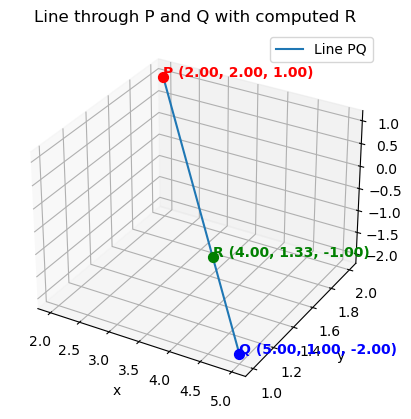
\includegraphics[width=0.7\columnwidth]{figs/line_3d.png}
    \caption{}
    \label{fig:placeholder}
\end{figure}



\end{document}
